\section{Study Design}
\label{sec:design}

\subsection{Overview}


\begin{figure*}[t]
    \centering
    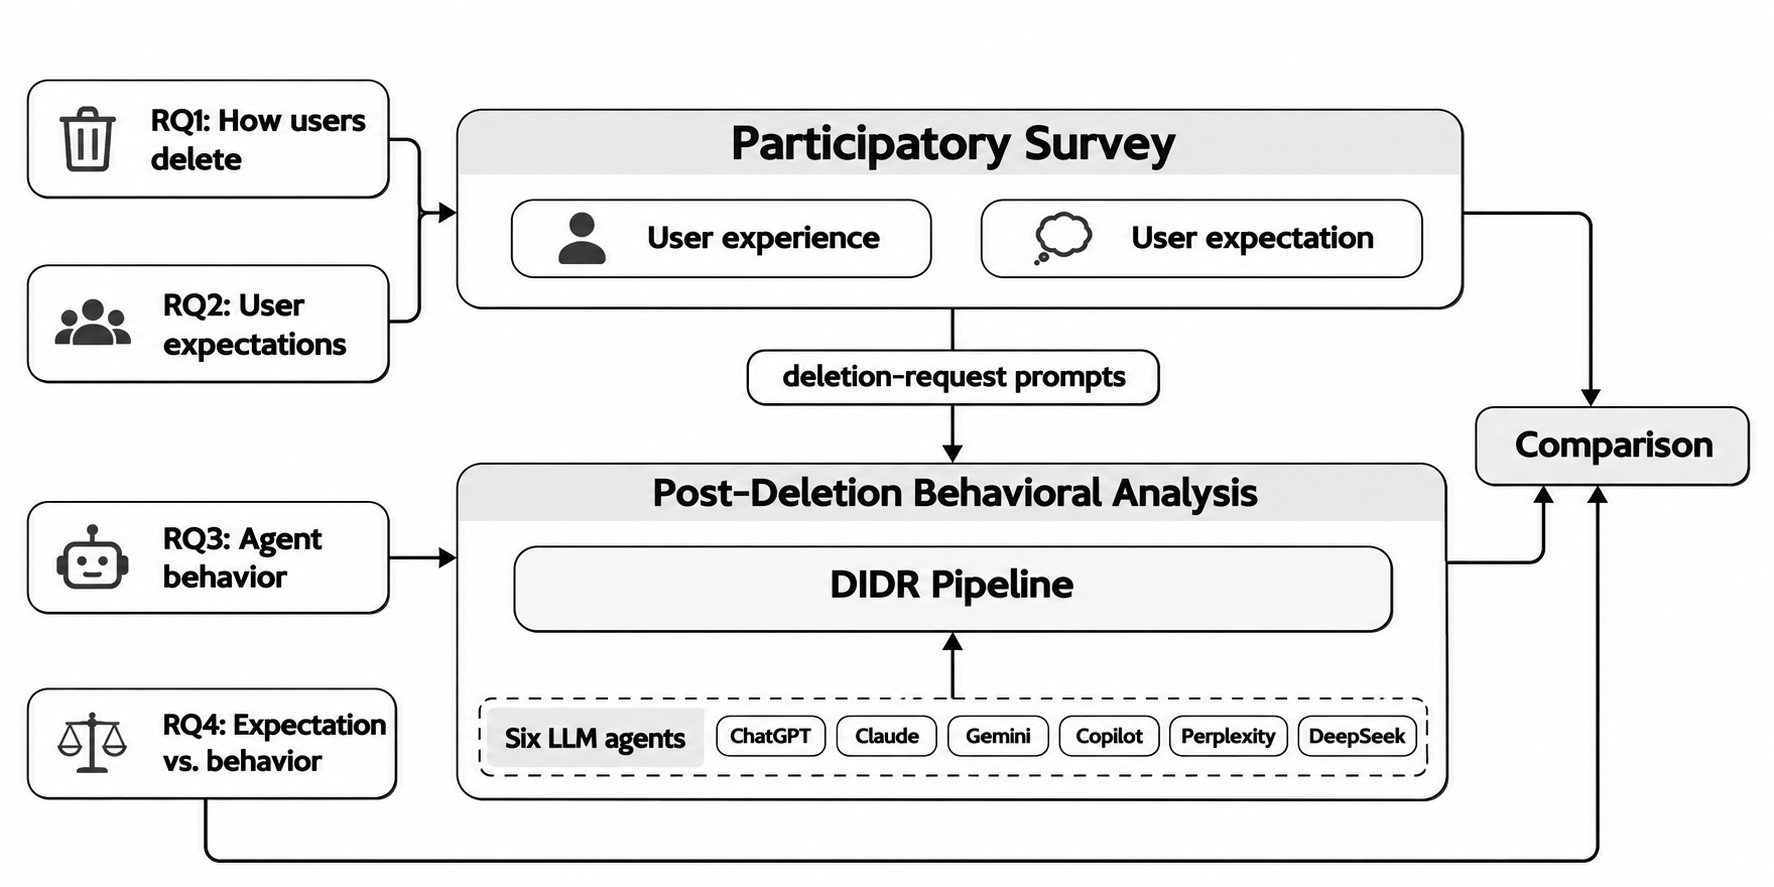
\includegraphics[width=0.9\textwidth]{figures/high-level.png}
    \caption{Overview of the study. The participatory survey answers RQ1 and RQ2, and its deletion requests feed the Post-Deletion Behavioral Analysis, which answers RQ3. Comparing the two answers RQ4.}
    \label{fig:overview}
\end{figure*}

We examine data deletion in commercial LLM agents from two complementary perspectives: users' expectations and agents' post-deletion behavior (Figure~\ref{fig:overview}). First, a participatory survey examines how users approach data deletion across two scenarios, including their choice of deletion method, deletion-request prompts, expectations, and verification strategies. We then use the collected deletion requests in a Post-Deletion Behavioral Analysis, where we inject synthetic facts into six commercial LLM agents, apply deletion methods, and subsequently probe for data recall. Finally, we compare survey responses with observed agent behavior to identify discrepancies between users' expectations and what deletion achieves in practice.


Our four research questions follow this design. The survey answers RQ1 (How do users delete data from LLM agents, and does scenario sensitivity change what they do?) and RQ2 (What do users expect deletion to do, and how do they check that it worked?). The post-deletion analysis answers RQ3 (What do agents do after a deletion request, and how do they differ from each other?). Only the two together answer RQ4 (Where do user expectations and agent behavior differ?).


\subsection{Participatory Survey}

\subsubsection{Participant recruitment}

We recruited U.S. adults through Prolific who had used at least one of the six LLM agents described in Section~\ref{sec:background}. The survey was administered through Qualtrics, with a recruitment target of approximately 200 participants rather than a power-based sample size. Participants received \$4 each.

Of 235 submissions, 17 were incomplete and one failed an attention check. We excluded another 36 respondents who reported no prior experience deleting data from an LLM agent, as the survey examined deletion practices and expectations among users with such experience. Of the remaining 181 participants, four did not complete the method-choice question in both scenarios, yielding a final survey sample of 177. Separately, deletion-request prompts for the Post-Deletion Behavioral Analysis were drawn from 209 participants, including those without prior deletion experience, because the request-writing task was hypothetical (Section~\ref{sec:didr}).

Among the 177 participants, 73.4\% were under 45, and 62.1\% held at least a bachelor's degree (Appendix~A). Our findings therefore characterize users with prior deletion experience rather than the broader population of LLM-agent users.

\subsubsection{Survey design}

To address RQ1 and RQ2, we designed a survey examining users' deletion practices, perceptions of deletion methods, expectations, and verification strategies. Participants evaluated two scenarios differing in data sensitivity. The less sensitive scenario involved sharing a city while requesting weather information, while the more sensitive scenario involved disclosing a home address when seeking a clinic for a sexually transmitted infection. In both scenarios, participants considered deleting the shared location data. The scenarios used identical questions and were presented in randomized order to mitigate order effects. The survey used the term ``AI chatbot'' to refer to LLM agents.

Participants first indicated which of eight deletion methods they had previously used: the six listed in Table~\ref{tab:methods}, account deletion, and filing a deletion request. In each scenario, they selected a method from those previously used and rated its perceived protection, effort, and benefit loss using five-point agreement scales comprising five, four, and three items, respectively. They also selected a preferred method from all eight options, regardless of prior experience. Additional questions assessed willingness to delete, expected deletion outcomes, and verification practices. Participants then wrote the deletion request they would send to the agent.

Before the scenarios, participants reported which LLM agents they had used and their duration of use. Following the scenarios, they answered questions about prior deletion experiences, including the types of data they had attempted to delete, their motivations, and whether deleted information had resurfaced. The survey concluded with a privacy-knowledge quiz, questions about attitudes toward LLM agents and data sharing, and demographic questions. Two instructed-response items served as attention checks. Appendix~B provides the complete scenarios, measurement items, and attention checks.

\subsubsection{Data analysis}

We report percentages of the 177 participants, within each scenario or with both scenarios combined. When the scenarios are combined, a response is one participant's answer in one scenario, and percentages are of responses. Each participant answered in both scenarios, so we compare the scenarios within participants. For the five-point ratings we use Wilcoxon signed-rank tests, because a normality test rejected normality of the differences. For choices, such as the method chosen or the options marked, we use McNemar tests, which suit the same participant choosing in both scenarios.

To compare methods, we use only the four methods chosen by at least 14 participants, because smaller groups are too small to compare. Where we combine both scenarios, each participant contributes two responses, so we use models that account for that (generalized estimating equations clustered by participant). There are 354 responses in all, fewer where a participant chose Other or the method has too few participants. To check that protection, effort, and benefit loss measure separate things, we ran a confirmatory factor analysis (Appendix~C).

Because we ran many tests on a modest sample, the analyses are exploratory. We adjust $p$ values for the number of tests (Holm correction, reported as $p_{\mathrm{Holm}}$; unadjusted values are $p$). A nonsignificant result means we found no association, not that none exists. Table~\ref{tab:analysis-families} in the Appendix lists each analysis, its test, and its correction family. The written deletion requests are coded and sampled in the post-deletion analysis (Section~\ref{sec:didr}), not here.

\subsection{Post-Deletion Behavioral Analysis}
\label{sec:didr}

\begin{outlinenote}
start with a leading paragraph, and figure, as overview of these steps
\begin{itemize}[leftmargin=*,nosep]
\item Say that we built a new data injection, deletion, and recall pipeline, DIDR Pipeline)
\item talk to the figure that make the steps and relationships between the components clear
\item components in the figure (and pipeline):
\begin{itemize}[leftmargin=*,nosep]
\item[(1)] input: commercial LLM agents
\item[(2)] synthetic fact generation (define fact as a <entity, attribute, value> tuple)
\item[(3)] data injection
\begin{itemize}[leftmargin=*,nosep]
\item[(3.1)] synthetic fact injection
\begin{itemize}[leftmargin=*,nosep]
\item through prompts
\item through UI actions
\end{itemize}
\end{itemize}
\item[(4)] data deletion
\begin{itemize}[leftmargin=*,nosep]
\item[(4.1)] input: deletion-request prompts (from survey)
\item[(4.2)] stratified prompt sampling (this will include coding, purpose is to identify the most representative prompts, and reduce redundant testing)
\item[(4.3)] input: deletion-request UI actions
\item[(4.4)] issue deletion requests
\begin{itemize}[leftmargin=*,nosep]
\item through prompts
\item through UI actions
\end{itemize}
\end{itemize}
\item[] \-\-> 31 days
\item[(5)] data recall
\begin{itemize}[leftmargin=*,nosep]
\item[(5.1)] prompt-based recall (direct recall prompt, which is asking about entity and attribute, indirect recall prompt, which is asking about only the entity)
\item[(5.2)] UI-based check
\end{itemize}
\end{itemize}
\item implementation: playwright-based automation (in the figure, this should underlie or connect to injection, deletion, and recall as they all need this).
\end{itemize}
\end{outlinenote}

To observe what agents do after a deletion request, we built a pipeline that injects a known fact into an agent, deletes it, and later tests whether the agent still returns it: the data injection, deletion, and recall (DIDR) pipeline (Figure~\ref{fig:didr}). Because we plant the fact ourselves, we know exactly what the agent was told, and a later recall can be traced back to it. Each test case combines one fact, one way of injecting and deleting it, and one agent. The pipeline starts with synthetic fact generation, which produces the facts we inject into commercial LLM agents. The pipeline runs in two parts. Through UI actions, we walk through each agent's interface and inject and delete facts in every way it offers, from typing in the chat to using memory pages and history controls. Through prompts, we inject a fact with a conversational disclosure and delete it with a deletion request that a participant wrote in the survey. In both parts, we delete at least 48 hours after injection, so the agent has time to process the fact, and we run data recall at least 30 days after deletion, so that the up to 30 days some agents document for deleted data have passed. Data recall tests whether the agent still returns the fact, through recall prompts and a UI-based check. Playwright-based automation drives the three stages where a control can be automated, and we ran the others by hand (for example Gemini's activity deletion, where we chose a time frame that held the injection).
    
\begin{figure*}[t]
    \centering
    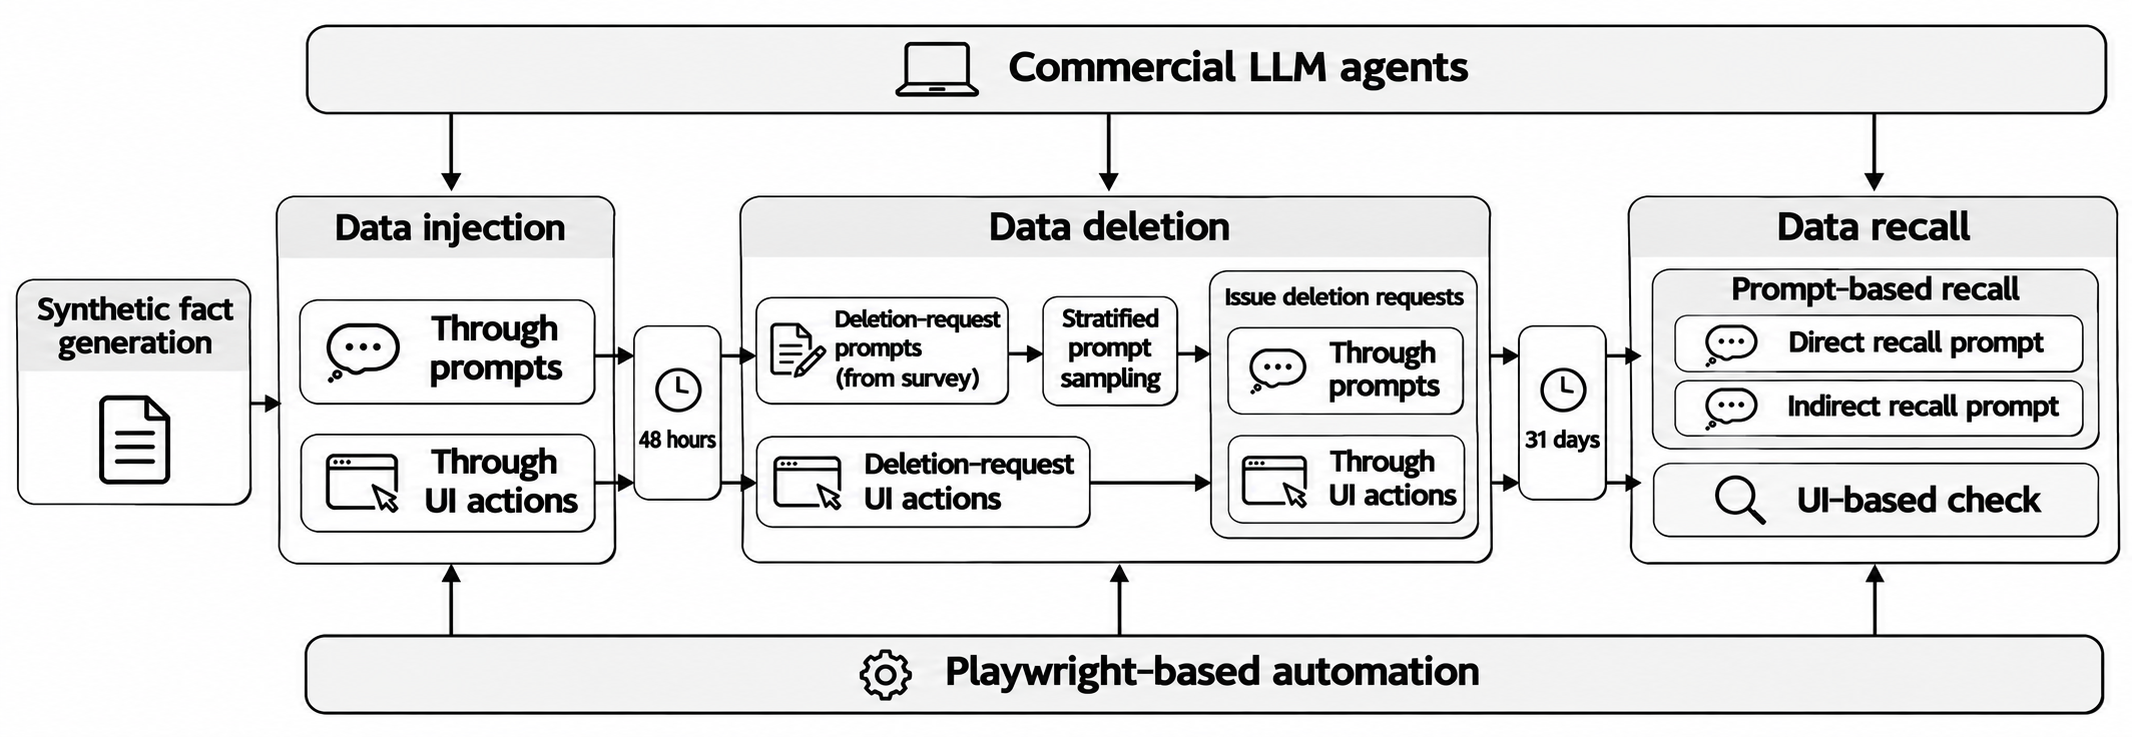
\includegraphics[width=\textwidth]{figures/DIDR.png}
    \caption{The DIDR pipeline. Synthetic facts are injected into commercial LLM agents, followed by deletion at least 48 hours later and recall testing at least 30 days after deletion. Each stage uses prompt-based and UI-based interactions, automated with Playwright.}
    \label{fig:didr}
\end{figure*}

\para{Synthetic fact generation}

To trace any later recall to the fact that caused it, each test case needs a fact the agent could not already know. We therefore generate synthetic facts, each a tuple of an entity, an attribute, and a value. The entity is an ordinary thing a person might mention in passing, such as a scarf being knitted or a sourdough starter. The attribute is its name. The value is a made-up code name of two to four words. For example, one fact is $\langle$a scarf I'm knitting, name, ``Magnifier King Broom''$\rangle$. Each value is unique to one test case, following the canary approach of Carlini et al.~\cite{carlini2019secret}, so a recall of the value identifies the test case it came from. We wrote the entities ourselves, from curated lists of everyday objects and projects. We drew each value from the EFF long word list, kept only words with a noun sense in WordNet, and removed words under WordNet's weapon, drug, and sexual-content categories, along with a short list of other terms, because content that a platform's safety filter might intercept would confuse a filtered answer with a deleted fact. Each fact is delivered in a casual sentence that varies across test cases, because a single repeated template would look unlike real chat.

\para{Data injection}

We inject each fact in the ways people put information into agents, and we use more than one because each reaches a different place where an agent may keep it. Through UI actions, we inject each fact in every way the agent's interface allows: mentioned in passing in a conversation, as an explicit request to remember it, or entered on a page such as a memory page, custom instructions, or Gemini's saved-info page. We found these by walking through each agent's web interface and listing every way a user can put information in, an approach similar to earlier walkthroughs of LLM privacy controls~\cite{li2026privacy}. Where an agent offers only some of these, we use those. Through prompts, every fact is a casual sentence mentioned in passing in a chat, always the same way in, so injection is held constant and only the deletion request varies. Deletion follows at least 48 hours after injection, which gives the agent time to process the fact, such as saving it to memory, before we delete it.

\para{Data deletion}

Through UI actions, we use the methods we found in the walkthrough, which match the controls users actually have and the methods our survey participants know (Table~\ref{tab:methods}). One of these methods, sending a deletion-request prompt, is typed in the chat, so 13 of the test cases through UI actions are typed requests. Each acts on a place where an agent may keep the fact, such as the conversation, individual or all saved memories, a saved-info page, activity history, or a privacy dashboard. For each agent we also ran the most extensive deletion, a combination of all its controls and the most a careful user could do, to see whether anything still comes back. We did not test two of the survey's eight methods: deleting the account, because nothing is left to observe once the account is gone, and filing a request with the company, because it is handled outside the agent where we cannot observe the result. We also left out settings that only switch a feature off, because they stop future collection and delete nothing already stored. Test cases whose deletion could affect other test cases, such as account-wide actions, ran on dedicated accounts, and deletions that share an account ran from narrowest to broadest. This keeps each result tied to the method under test: otherwise an account-wide deletion run for one test case could clear the fact in another test case that was still waiting for its own deletion or recall, and we could not tell which deletion removed it. This gives 73 test cases through UI actions across the six agents, of which we could run 67, because six Perplexity controls need a paid plan.

Through prompts, we take the deletion requests from the survey so that they match how users actually ask. In total, 209 participants wrote 415 requests, including participants without deletion experience, because the task was hypothetical. After removing repeats and duplicates, 375 distinct requests remained, and we redacted identifying details from 7 of them. Testing all 375 on six agents would have meant 2,250 test cases under free-tier rate limits, so we tested a sample chosen to be representative and to avoid redundant tests. We grouped the requests into seven groups with keyword rules, for example whether a request mentions memory, the conversation, the account, or a database, and drew 138 requests by stratified random sampling, with at least 15 per group so the two smallest groups were included in full. The groups only spread the sample and are not used in any analysis. Two researchers then independently coded the 138 requests on seven dimensions of wording, such as where a request asks to delete and how politely it is phrased, so that we can test whether wording affects the outcome. Their agreement was high (Gwet's AC1 of 0.954 pooled over the seven dimensions; Appendix~D). Five requests asked to delete all of a user's data and could have deleted other test cases' facts, so we excluded them. We sent the remaining 133 to all six agents after injecting a fact through a prompt, which gives 798 test cases. Together with the 67 test cases through UI actions, we ran 865 test cases. We also tested uploaded files as a separate group of 12 test cases, deleting the conversation and applying the most extensive deletion on each agent, because an agent can read an uploaded document, save it to memory, do both, or do neither. Every deletion in this group was a button, so there is no reply to code, and we report the 11 we could run one by one. The most extensive deletion on Perplexity needs a paid plan.

\begin{outlinenote}
just use multiple paragraphs if we need it, but don't need to highlight the other paragraphs
\end{outlinenote}

\para{Data recall}

We wait at least 30 days after deletion because ChatGPT, Claude, and Perplexity document that deleted data can persist in their systems for up to 30 days, and the same minimum wait for all six agents keeps the results comparable. We then test whether the agent still returns the value, through prompt-based recall and a UI-based check. Prompt-based recall opens a new conversation. A direct recall prompt asks about the entity and the attribute, as a user trying to find out whether something was kept would. A direct prompt alone is not enough, because an agent can hold information and not volunteer it. An indirect recall prompt therefore asks for an ordinary task about the entity and does not name the attribute or contain the value, which tests whether the fact surfaces in the output a user would actually see. We send each of the two prompts twice with different wording, because replies vary between runs and one miss could be chance. We check whether each reply contains the value and review all replies by hand. The UI-based check reads the memory or saved-info page the agent shows its users. It does not depend on the agent's reply, so it can show that an entry is still stored when the agent says nothing. It applies only where the agent has such a page, so it is not used for DeepSeek or Perplexity, and not on the Copilot accounts that lacked the page.

 We run the UI-based check first, then the indirect recall prompt, then the direct recall prompt, so the direct prompt, which names the entity, cannot influence the other checks. A test case is a recall success if any check returns the value. It is recall failed only when no check does and the fact is known to have reached the place we tested. Otherwise it is can't tell, so that a missing answer is never counted as proof of deletion. We count the fact as having reached the place we tested only when the agent showed or said that it saved it: its interface displayed a memory notice such as ``Memory updated'', or its reply said in storage words that it had saved the fact. A reply that only reacts to the fact, such as ``Got it'', no signal at all, or a statement that the agent cannot store it does not count. We read this from the reply and the screenshot saved at injection, and settled unclear replies by hand. When a deletion request was typed into the original conversation, we also send the first direct prompt back in that conversation, and report it separately, because the original disclosure is still in that chat's context.

For deletions through UI actions, we also coded whether the interface changed: whether the screen the action acts on showed the fact gone afterwards, such as a conversation missing from the history list or an entry missing from a memory page. We coded this from the screenshot taken after the deletion and, where it did not show the result, checked the account directly. A deletion typed into the chat leaves nothing on the interface to inspect, so its interface change is not observable.

To judge whether what we found matches what an agent promises, we assigned each test case a commitment type from the agent's own published help and privacy pages, for the deletion method and the place the fact was injected. A commitment is deletes when the documentation says the method removes the content, does not delete when it says the method does not reach it, no commitment when it is silent, unrelated when the method does not apply to where the fact was injected, and not testable when the account could not reach that place. Only deletes and does not delete support a verdict. For a deletes commitment, a recall success or an unchanged interface contradicts it, and a recall failed with an interface that changed or is not observable is consistent with it, and where the documentation says past conversations remain, recall success from those conversations alone is consistent with it. For a does not delete commitment, recall success is consistent with it. Every other test case, including can't tell, stays unresolved. For the other three commitment types we report the recall result without comparing it to the documentation, because it states nothing to compare against.

We also coded what the agent said in reply to each deletion request typed in the chat. Two researchers independently coded each reply as complied, partial, deflected, refused, silently ignored, or other (Appendix~D), judging only what the agent said and not whether anything was deleted. Their agreement was high (Gwet's AC1 of 0.969 on 788 replies), and we settled disagreements by discussion. Deletions through UI actions have no reply to code.

We also counted recall replies that decline to give the fact because the user earlier asked the agent to delete it or not use it. We found these by matching phrases that cite the earlier request, and we checked every match by hand for ChatGPT and Perplexity, the only agents with matches. These replies do not change the outcome: a reply that does not give the fact is still scored by the rule above.

To test whether wording affects the outcome, we compare recall success across the codes of each dimension for each agent. Because some codes hold few deletion requests, we report counts and give no tests, and we look only at codes with at least six deletion requests. We leave out agents whose test cases are all can't tell.

\para{Comparing expectations with behavior}
To find where expectations and behavior differ, we take each data deletion method that participants chose in the survey and look at the test cases that used the same method. The survey percentages are shares of participants' responses and the post-deletion percentages are shares of test cases, so we do not compare the two numbers directly. We ask instead whether what participants expected held up in the post-deletion analysis. We make two comparisons. We set what participants expected deletion to do against whether the fact came back, which is recall success, and we set the checks participants said they used, asking the agent in the same conversation and looking at whether the interface changed, against what those checks showed in our test cases.
